\documentclass{article}

\usepackage[utf8]{inputenc}
\usepackage[french]{babel}
\usepackage[a4paper, left=2cm, right=2cm, top=2.5cm, bottom=2.5cm]{geometry}
\usepackage{amssymb}
\usepackage{amsmath}
\usepackage{graphicx} % pour les images 
\usepackage{listings} % pour intégrer un code R
\usepackage{xcolor} % pour coloriser le code R intégré
\usepackage{comment}
\usepackage{float}
\usepackage{amsthm}


\theoremstyle{plain}
\newtheorem{definition}{Définition}[section]

\theoremstyle{definition}
\newtheorem{example}[definition]{Exemple}
\newtheorem{remark}[definition]{Remarque}

\theoremstyle{plain}
\newtheorem{theorem}[definition]{Théorème}
\newtheorem{lemma}[definition]{Lemme}
\newtheorem{proposition}[definition]{Proposition}



\lstset{
	language=R,
	inputencoding=utf8, 
	extendedchars=true,       
	basicstyle=\ttfamily\footnotesize,
	keywordstyle=\color{blue},
	commentstyle=\color{green!50!black},
	stringstyle=\color{red},
	numbers=left,
	numberstyle=\tiny,
	stepnumber=1,
	breaklines=true,
	literate=%
	{é}{{\'e}}1
	{è}{{\`e}}1
	{ê}{{\^e}}1
	{à}{{\`a}}1
	{ù}{{\`u}}1
	{ç}{{\c{c}}}1
}

\title{Étude des valeurs extrêmes univariées}
\author{El Mazzouji Wahel, Mariac Damien, Condamy Fabian} 
\date{\today} 

\begin{document}

\maketitle 
\newpage
\tableofcontents 
\newpage
\section{Introduction}
Les événements extrêmes, comme les crues majeures, les canicules intenses ou les krachs financiers, sont rares mais peuvent avoir des conséquences très importantes. Les étudier est devenu essentiel dans des domaines variés comme la climatologie, l’assurance, la finance ou encore l’ingénierie.

\noindent La théorie des valeurs extrêmes est un outil statistique qui permet de modéliser ces phénomènes rares, en se concentrant sur les valeurs situées aux extrémités d’un jeu de données : les plus grandes ou les plus petites. Contrairement aux méthodes classiques qui s'intéressent surtout à la moyenne ou à la variance, la théorie des valeurs extrêmes cherche à comprendre le comportement des valeurs extrêmes.

\noindent Dans les statistiques classiques, beaucoup de résultats reposent sur le théorème central limite, qui explique que, sous certaines conditions, la moyenne d’un grand nombre de variables aléatoires suit une loi normale. C’est un fondement de nombreuses méthodes, mais il ne dit rien sur les valeurs les plus extrêmes d’un échantillon, qui sont pourtant cruciales dans l’analyse du risque.

\noindent Cette théorie s’intéresse donc à des grandeurs comme le maximum d’un échantillon $(X_1, X_2, \dots, X_n)$~:
\[
M_n = \max\{X_1, X_2, \dots, X_n\}.
\]

On cherche à savoir si, en normalisant ce maximum, il converge vers une loi limite. Les travaux de Fréchet, Fisher, Tippett et Gnedenko ont montré que cette convergence est possible, et qu’il n’existe que trois lois limites possibles : la loi de Fréchet, la loi de Gumbel et la loi de Weibull, qui correspondent à différents types de comportements des queues de distribution.
En s’intéressant aux comportements les plus rares, la théorie des valeurs extrêmes fournit un cadre rigoureux pour mieux anticiper l’intensité et la fréquence des événements extrêmes, et ainsi mieux s’y préparer.
\section{Comportement asymptotique de $M_n$}

\subsection{Caractérisation avec la fonction de répartition}

On commence par faire une remarque sur la fonction de repartion de $M_n$ en utilisant le fait que les $X_i$ sont i.i.d.
En effet, si on note $F_{M_n}$ la fonction de repartition de $M_n$, et $F$ la fonction de repartition de $X_i$ on a :
\[
\forall t \in \mathbb{R} , \quad F_{M_n}(t) = \mathbb{P}(M_n \le t) = \mathbb{P}(X_1 \le t,...,X_n \le t)=\mathbb{P}(X_1 \le t)^n = F_{X_1}^n(t) 
\]
\\
On remarque que, pour tout $t$ strictement inférieur à $t^*$ la borne supérieure du support des $X_i$, on a $F(t)<1$ et donc
\[
F(t)^n \xrightarrow[n\to +\infty]{} 0,
\]
et dans le cas ou t est supérieur ou égal à $t^*$, on a
\[
F(t)^n \xrightarrow[n\to +\infty]{} 1.
\]
L'idée est donc d'introduire deux suites ($b_n$) et ($a_n$) (avec $a_n > $  0 pour tout $n$) afin d'avoir une limite non dégénérée pour $\frac{M_n - b_n}{a_n}$. Comme la fonction de répartition caractérise la loi, il nous suffit d'étudier la fonction $G$ définie pour tout $t$ dans le support des $X_i$ comme :

\[
\mathbb{P} \left( \frac{M_n - b_n}{a_n} \le t \right) \xrightarrow[n\to +\infty]{} G(t)
\]
\\
S'il existe de telle suites $a_n$ et $b_n$, on dit que $F$ est dans le domaine d'attraction de $G$.
\\
\\
Il nous faut donc trouver les distributions $G$ qui peuvent apparaître comme limite dans l’équation ci-dessus.
\\
\\
Pour ce faire, nous utilisons cette définition de la convergence en loi :
\\
\\
\begin{definition}
\textbf{(Convergence en loi)}:
Soit \( Y_n \) une variable aléatoire de fonction de répartition \( F_n \), et soit \( Y \) une variable aléatoire de fonction de répartition \( F \).  
Alors $Y_n \xrightarrow{\mathcal{L} } Y$ si et seulement si pour toute fonction $z$ réelle, bornée et continue :
\[
\mathbb{E}[z(Y_n)] \xrightarrow[n\to +\infty]{} \mathbb{E}[z(Y)].
\]
\end{definition}
\noindent En prenant ici $Y_n = \frac{M_n -b_n}{a_n}$, on obtient :
\[
\mathbb{E}[z(\frac{M_n -b_n}{a_n})] = \int_{-\infty}^{\infty} z(\frac{x-b_n}{a_n}) \: n \:  F^{n-1} (x)dF(x)
\]
\\
\\
L'astuce ici va être de faire un changement de variable. On introduit alors la fonction quantile qui est définie par :
\\
\[
Q(p) \;=\; F^{-1}(p)
\;=\;
\inf\bigl\{x\in\mathbb{R}\,\bigm|\,F(x)\ge p\bigr\},
\quad p\in[0,1].
\]
\medskip 
\noindent On pose alors le changement de variable : 

\[
x = Q(1-\frac{1}{y}) = U(y) \; \; \; \; \; \; \text{et on obtient}
\]

\begin{equation}\label{eq:1.1}
    \int_{-\infty}^{\infty} z\Bigl(\frac{x-b_n}{a_n}\Bigr) \, n \, F^{n-1}(x)\,dF(x)
    =\int_{0}^{n} z\Bigl(\frac{U\Bigl(\frac{n}{v}\Bigr)-b_n}{a_n}\Bigr)
    \Bigl(1-\frac{v}{n}\Bigr)^{n-1}dv.
\end{equation}
\\
\\
Or, on a $\lim_{n \to \infty} ( 1 - \frac{v}{n})^{n-1} = e^{-v}$ , et on a $\lim_{n \to \infty} \mathbf{1}_{[0;n]}(x) = \mathbb{R}_{+}$.
\\
\\
Remarquons que, pour tout $t\in\mathbb R$, la probabilité
\[
\mathbb{P}  \Bigl(\frac{M_n - b_n}{a_n} \le t\Bigr)
\;=\;
\mathbb{P} \bigl(M_n \le a_n\,t + b_n\bigr)
\;=\;
F\bigl(a_n\,t + b_n\bigr)^{n}.
\]
Ainsi, la convergence en loi 
\[
\frac{M_n - b_n}{a_n}\;\overset{\mathcal{L}}{\xrightarrow[n\to +\infty]{}}\;Y
\quad\Longleftrightarrow\quad
\mathbb{P} \bigl(M_n \le a_n\,t + b_n\bigr)
\;\xrightarrow[n\to +\infty]{};
G(t),
\]
se traduit exactement par
\[
F\bigl(a_n t + b_n\bigr)^{n}
\;\xrightarrow[n\to\infty]{}\;
G(t).
\]
L'objectif est alors de trouver des expressions explicites pour les suites \(a_n\) et \(b_n\).

\subsection{Le paramètre $b_n$}

\noindent En reprenant l'expression ci-dessus et en passant au logarithme, on obtient :

\[
n \: \ln (F(a_n t + b_n)) \xrightarrow[n\to +\infty]{} \ln (G(t))
\]
\[
\text{Ce qui donne} \; \; n(- F(a_n t + b_n) + 1) \xrightarrow[n\to +\infty]{} \ln (G(t))
\]
En utilisant le développement limité de la fonction logarithme. 
\\
Le cas particulier de cette convergence pour $t=0$ donne :
\[
n\bigl(F(b_n)-1\bigr)\;\xrightarrow[n\to\infty]{}\;\ln G(0)
\;=\;-\,\ln G(0)\quad(\text{puisque }G(0)\in(0,1)),
\]
Comme on souhaite une limite non-dégénérée, on impose
\[
n\bigl[1 - F(b_n)\bigr] \;=\; 1.
\]
Il vient alors
\[
F(b_n)=1-\frac1n
\quad\Longleftrightarrow\quad
b_n \;=\; Q\!\Bigl(1-\tfrac1n\Bigr)
\;=\;U(n),
\]


\subsection{Le paramètre $a_n$}
Une fois la suite $(b_n)$ fixée comme précédemment, nous devons maintenant déterminer la suite $(a_n)$. L’objectif est de trouver des
 conditions suffisantes sur la fonction de répartition $F$ pour garantir l’existence d’une loi limite non dégénérée de $\frac{M_n - b_n}{a_n}$.
\\
\\
La convergence de $F^n(a_n t + b_n)$ vers une loi limite $G(t)$ est équivalente, par passage aux fonctions réciproques, à l’étude de la convergence de l’expression suivante :

\[
\lim_{x \to \infty} \frac{U(x/u) - U(x)}{a(x)} = h(u),
\]

Cette condition traduit, en quelque sorte, une régularité asymptotique de la queue de distribution.

\vspace{0.3cm}
\noindent
Nous avons alors la proposition suivante :

\begin{proposition}[Limites possibles de la fonction $h$]
Les fonctions limites possibles sont données, pour une certaine constante $c > 0$, par :
\[
c \cdot h_\gamma(u) = c \int_1^u v^{-\gamma - 1} \, dv = \frac{c(u^\gamma - 1)}{\gamma}.
\tag{2}
\]

Nous interprétons la fonction limite dans le cas $\gamma = 0$ par passage à la limite :
\[
h_0(u) = \log(u).
\]
\end{proposition}

\noindent
\textbf{Remarque.} La constante $c$ ne peut pas être nulle, car cela conduirait à une limite dégénérée pour la variable normalisée $\frac{M_n - b_n}{a_n}$. En pratique, on peut toujours ramener le cas $c > 0$ au cas $c = 1$ en absorbant $c$ dans la définition de la fonction $a$.
\\
\begin{proof} 
Soient $u,v >0$. Alors :
\[
\frac{U(xuv) - U(x)}{a(x)} 
\;=\; 
\frac{U(xuv) - U(xu)}{a(xu)} \,\frac{a(xu)}{a(x)}
\;+\;
\frac{U(xu) - U(x)}{a(x)}.
\tag{3}
\]
Si la limite dans $F$ est dans le domaine d'attraction de $G$ (\textit{ce qu'on suppose depuis le début}), alors le rapport $\frac{a(ux)}{a(x)}$ converge vers une fonction notée $g(u)$.
\\
\\
De plus,
\[
\frac{a(xuv)}{a(x)} 
\;=\;
\frac{a(xuv)}{a(xv)} \,\frac{a(xv)}{a(x)}.
\]
Par passage à la limite pour $x$, la fonction $g$ satisfait l'\textit{équation fonctionnelle de Cauchy} :
\[
g(uv) = g(u)\,g(v).
\]
\\
Les solutions de cette équation sont de la forme $g(u)= u^{\gamma}$ avec $\gamma$ un réel.
\\
Donc, on a $\lim_{x\to \infty} \frac{a(ux)}{a(x)} \;=\; x^{\gamma} l(x)$, on dit dans ce cas que $a$ est une fonction à variation régulière.
\\
\\
En réécrivant l'expression (2.3) avec cette convergence, on en déduit que la fonction limite est de la forme
\[
h_\gamma(u)= c\,\frac{u^\gamma-1}{\gamma},
\]
avec la convention \(h_0(u)=\ln u\).
\\
Ainsi, nous concluons que
\[
h_\gamma(u)=\frac{u^\gamma-1}{\gamma} \quad \text{(avec \(h_0(u)=\ln u\))},
\]
\end{proof}
\subsection{Les lois limites}
En reprenant $(3)$ et en utilisant ce qui précède, on obtient :
\[
\lim_{x\to \infty} \frac{U(xuv) - U(x)}{a(x)} = u^{\gamma} h(v) + h(u)
\]
\[
\text{autrement dit :} \; \; h_{\gamma}(uv)= u^{\gamma} h_{\gamma}(v) + h_{\gamma}(u)
\]
En reprenant le résultat de la proposition 2.2 et ce qui précède  $(2)$, on obtient :
\[
h_\gamma\Bigl(\frac{1}{v}\Bigr)=\frac{(1/v)^\gamma-1}{\gamma}=\frac{v^{-\gamma}-1}{\gamma}
\]
Posons \(u=\frac{v^{-\gamma}-1}{\gamma}\). On résout alors pour \(v\) :
\[
v^{-\gamma}=1+\gamma u\quad\Longrightarrow\quad v=(1+\gamma u)^{-1/\gamma}
\]
Le changement de variable de \(v\) à \(u\) permet de réécrire l'intégrale limite sous la forme
\[
\int_{u\in S_\gamma} z(u)\,d\Bigl\{\exp\Bigl[-\left(1+\gamma u\right)^{-1/\gamma}]\Bigr\}
\]
ce qui conduit à identifier la loi limite par
\[
G_\gamma(u)=\exp\Bigl\{-\left(1+\gamma u\right)^{-1/\gamma}\Bigr\}
\]
Il reste alors à étudier la nature du support \(S_\gamma\), mais celui-ci dépend du signe de \(\gamma\).
\\
On fait alors une disjonction de cas sur la valeur de $\gamma$.
\\
\\
\textbf{\underline{Cas si \(\gamma>0 : \)}}
\\
\\
L'inversion montre que \(v\in [0,1]\) correspond à \(u>-\frac{1}{\gamma}\).
\\
\\
De plus, pour de grandes valeurs \(x\) on a :
\[
S_{\gamma} \approx \exp\Bigl[-\bigl(1 + \gamma x\bigr)^{-1/\gamma}\Bigr]
\]
Or, par un développement asymptotique,  \(\bigl(1 + \gamma x\bigr)^{-1/\gamma}\) est proportionnel à \(x^{-1/\gamma}\) pour \(x\) grand. On obtient alors
\[
S_{\gamma} \approx \exp\bigl[-C\,x^{-1/\gamma}\bigr] 
\quad (\text{pour une constante } C>0).
\]
Par croissance comparé, comme \(x^{-1/\gamma}\) tend vers 0 moins vite que \(\exp(-\alpha x)\). On a alors : 
\[
S_{\gamma}\,\sim\, K\,x^{-1/\gamma} 
\quad (\text{pour } x\to\infty),
\]
ce qui caractérise une \textbf{queue lourde} : la probabilité d'observer des valeurs très grandes est plus élevée que dans un modèle à décroissance exponentielle.
\\
\\
\textbf{\underline{Cas si \(\gamma<0 : \)}}
\\
\\
Pour \(\gamma < 0\), la loi est définie si $1 + \gamma u > 0$ c'est à dire $u < - \frac{1}{\gamma}$. Cela signifie que la distribution a son support dans \(]-\infty, - \frac{1}{\gamma} [ \), et on pose alors \(x_{\max} = - \frac{1}{\gamma} \).
\\
Par conséquent, la fonction de survie $S_{\gamma} = 1 - G(x)$ = 0 pour \(x \ge - \frac{1}{\gamma} \).
\\
\\
Autrement dit, il n'y a aucune probabilité d'observer une valeur au-delà de \(x_{\max}\). Dans ce cas, on dit que la distribution est à \textbf{queue bornée}.
\\
\\
\textbf{\underline{Cas si \(\gamma=0 : \)}}
\\
\\
Lorsque \(\gamma = 0\), on a posé $h_0(u)=\ln u$.
\\
Donc, le changement de variable s'adapte : 
\[
u=h_0\Bigl(\frac{1}{v}\Bigr)=\ln\Bigl(\frac{1}{v}\Bigr)=-\ln v,
\]
ce qui implique
\[
v=e^{-u}.
\]
Le changement de variable transforme alors l'intégrale limite en
\[
\int_{-\infty}^{\infty} z(u)\,d\Bigl\{\exp\Bigl[-e^{-u}\Bigr]\Bigr\},
\]
et la loi limite est alors donnée par
\[
G_0(u)=\exp\Bigl\{-e^{-u}\Bigr\},\qquad u\in\mathbb{R},
\]
On retrouve ici une queue à décroissance exponentielle, ce qui est caractéristique d'une \textbf{queue légère} : la probabilité d'observer des valeurs extrêmes est faible mais pas impropable.
Il s'agit d'un cas intermédiaire entre les deux cas précédents.
\\
\subsection{Résumé}
Les lois limites sont les suivantes :
\\
\begin{itemize}
    \item Si \(\gamma>0\) (loi de Fréchet) :
    \[
    G_\gamma(u)=\exp\left\{-\left(1+\gamma u\right)^{-1/\gamma}\right\}, \quad u > -\frac{1}{\gamma}.
    \]
    
    \item Si \(\gamma=0\) (loi de Gumbel) :
    \[
    G_0(u)=\exp\left\{-e^{-u}\right\}, \quad u\in\mathbb{R}.
    \]
    
    \item Si \(\gamma<0\) (loi de Weibull) :
    \[
    G_\gamma(u)=\exp\left\{-\left(1+\gamma u\right)^{-1/\gamma}\right\}, \quad u < -\frac{1}{\gamma}.
    \]
\end{itemize}
On observe alors qu’apparaît un \textbf{modèle paramétrique} : la loi limite des maxima s’exprime selon une famille de lois qu’on appelle \emph{GEV} (Generalized Extreme Value), paramétrée par trois paramètres :

\begin{itemize}
  \item un paramètre de position $\mu$,
  \item un paramètre d’échelle $\sigma > 0$,
  \item un paramètre de forme $\gamma$.
\end{itemize}

Ils proviennent des suites de normalisation $a_n > 0$ et $b_n$ introduites dans l’étude de la variable normalisée \(\frac{M_n - b_n}{a_n}\). 

On pose alors $\mu = b_n \; \text{et} \; \sigma = a_n$, ce qui permet de réécrire la variable réduite \(u = \frac{x - \mu}{\sigma}\). Ainsi, la forme générale de la fonction de répartition limite devient :
\[
G_{\mu, \sigma, \gamma}(x) = \exp\left\{-\left[1 + \gamma \left(\frac{x - \mu}{\sigma} \right)\right]^{-1/\gamma} \right\}.
\]

Ce modèle permet donc d’ajuster statistiquement la loi des maxima à partir des données, en estimant directement ces trois paramètres.


\newpage
\section{Quelques exemples numériques}

\noindent Voici maintenant quelques applications numériques sur des lois usuelles de ce que nous avons vu dans cette section. Pour chacune des représentations suivantes, nous avons simulé $n=1000$ fois chaque loi puis ensuite effectué $N=10000$ simulations pour le maximum afin d'avoir une précision correcte. 

\subsubsection{Loi uniforme}

\noindent Pour la loi uniforme sur [0,1], on peut montrer théoriquement que la limite du max est une loi exponentielle de paramètre 1 (loi de Weibull bien particulière). \\
\noindent Soient \( U_1, U_2, \dots, U_n \) des variables aléatoires indépendantes et identiquement distribuées selon la loi uniforme sur \([0,1]\).

\noindent On a, pour $ x \in [0,1]$ :

\begin{align*}
	P(M_n \leq x) &= P(U_1 \leq x, \dots, U_n \leq x) \\
	&= P(U_1 \leq x)^n \text{ par indépendance des $U_i$}\\
	&= x^n
\end{align*}

\noindent Nous allons maintenant effectuer le changement de variable $ x = 1 - y/n $ avec $y > 0 $ pour examiner la queue de la distribution :

\[
P(M_n \leq 1 - y/n) = (1 - y/n)^n.
\]

\noindent De plus, on a: $(1 - y/n)^n \xrightarrow[n \to +\infty]{} e^{-y} $. Donc, $ P(M_n \leq 1 - y/n) \xrightarrow[n \to +\infty]{} e^{-y} $.


\noindent Or, par définition, la loi exponentielle de paramètre 1 a pour fonction de répartition : $ P(Y \leq y) = 1 - e^{-y}, \quad y > 0. $

\noindent Ainsi, on a donc montré que :

\[
P(n(1 - M_n) \leq y) \to P(Y \leq y) = 1 - e^{-y},
\]

\noindent ce qui établit la convergence en loi :

\[
Y_n = n(1 - M_n) \xrightarrow{\mathcal{L}} \mathcal{E}(1).
\] 
\noindent Ainsi, on prendra ici $a_n$ = $\frac{1}{n}$ et $b_n$ = 1.

\noindent Une simulation sur Rstudio donne le graphe suivant :

\begin{center}
	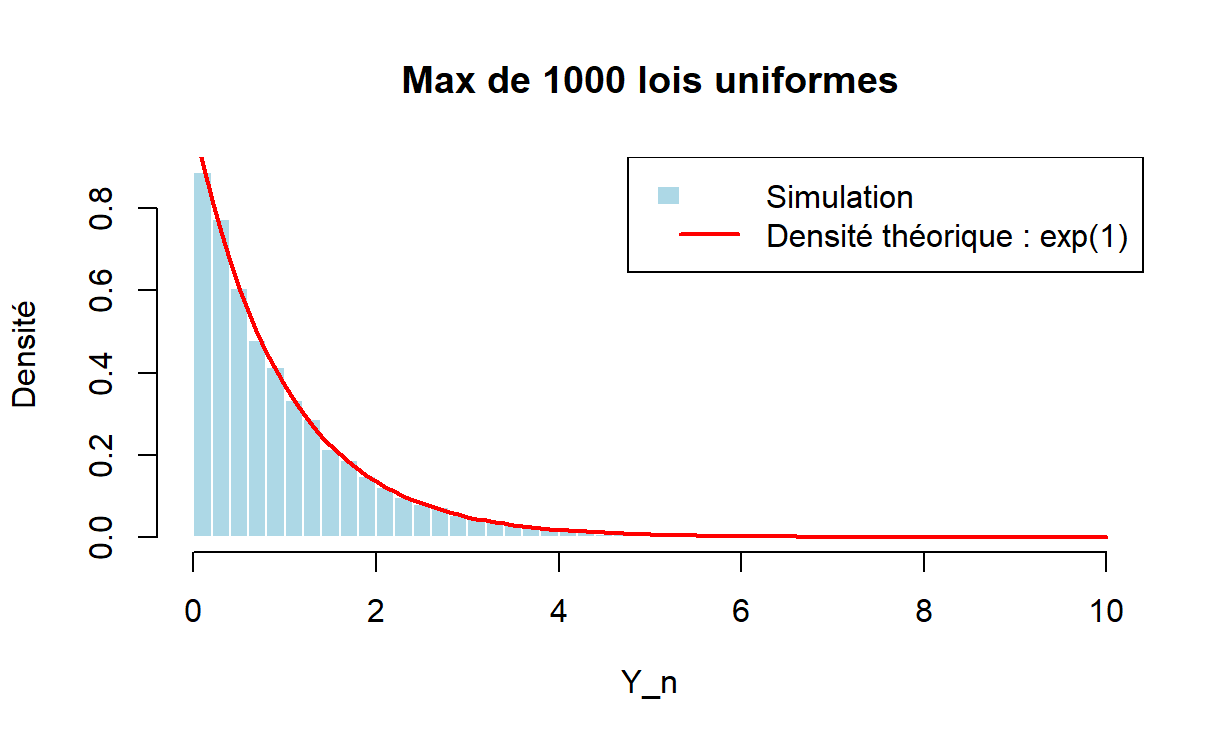
\includegraphics[scale=0.8]{./images/Max_Uniforme.png} 
\end{center}

\noindent Remarquons que l'on obtient une loi de Gumbel, ce qui est assez logique au vu du fait que ce soit une loi à queue très légère (elle n'en a tout simplement pas car son support est borné).

\subsubsection{Loi exponentielle}
\noindent Pour une loi exponentielle de paramètre 1, la loi limite est une loi de Gumbel. Théoriquement, on trouve $a_n = 1 $ et $b_n = \log(n) $. \\
\noindent En effet, soient $X_1, \dots, X_n$ des variables aléatoires iid de loi $\mathcal{E}(1)$. On a pour $ x \geq 0 $ :

\begin{align*}
	P(M_n \leq x) &= P(X_1 \leq x, \dots, X_n \leq x) \\
	&= P(X_1 \leq x)^n \\
	&= (1-\exp(- x))^n
\end{align*}

\noindent Passons donc à la normalisation, posons $z=\frac{x-b_n}{a_n}$, on va utiliser le fait que $(1-\exp(- x))^n \xrightarrow[x \to +\infty]{} \exp(-n\exp(-x)) $. \\
\noindent Ainsi on veut choisir $b_n$ de telle sorte que $n \exp(-b_n) \xrightarrow[n \to +\infty]{} 1 $. D'où $b_n = \log(n)$ \\
\noindent On a donc $ x = a_n z + \log(n) $. On peut donc choisir $ a_n = 1$ afin d'avoir : 
\begin{align*}
	P(\frac{M_n - \log(n)}{1} \leq z) &= (1 - \exp(-(z+\log(n))))^n \\
	&= (1 - \frac{\exp(-z)}{n})^n 
\end{align*}

\noindent Et donc : $ (1 - \frac{\exp(-z)}{n})^n \xrightarrow[n \to +\infty]{} \exp(\exp(-z))$ \\

\noindent Ainsi, on a bien montré que $\frac{M_n - \log(n)}{1} \xrightarrow{\mathcal{L}} \text{Gumbel}(0,1) $ \\

\noindent On obtient alors numériquement le graphe suivant :

\begin{center}
	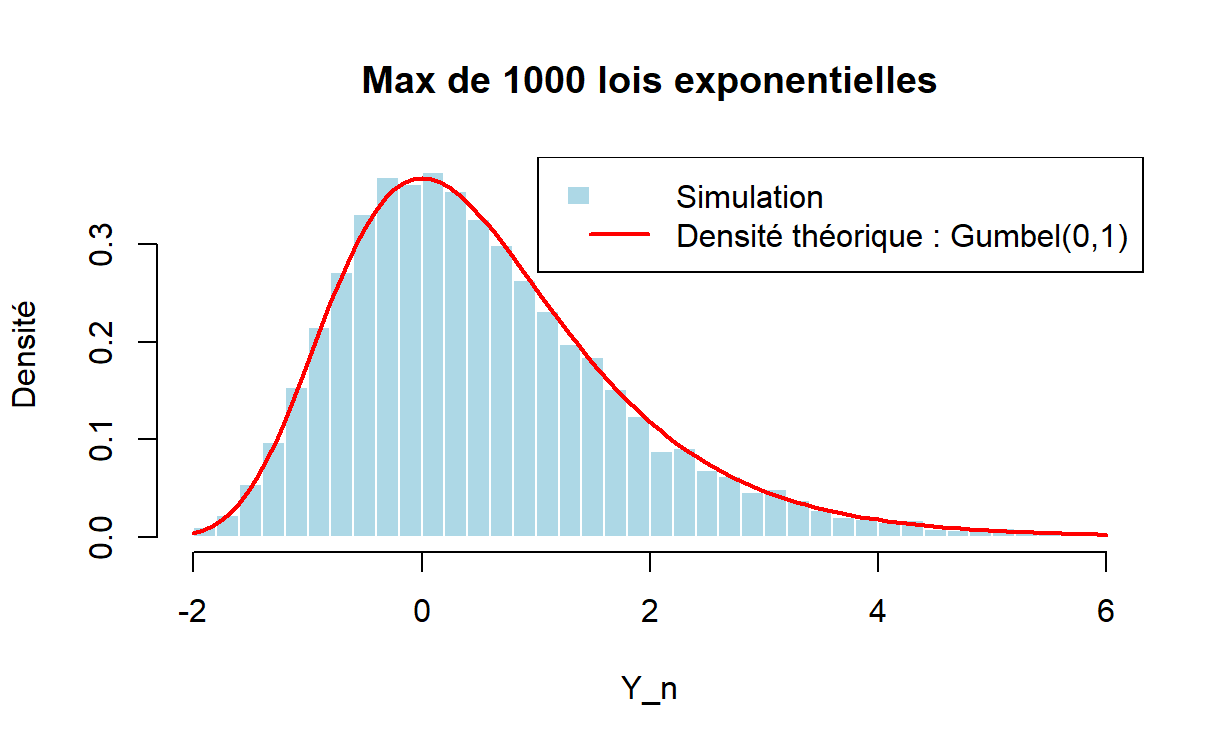
\includegraphics[scale=0.8]{./images/Max_Expo.png} 
\end{center}

\noindent Cette fois-ci, on avait une loi à queue fine, et on obtient loi de Gumbel, ce qui était attendu.

\subsubsection{Loi normale}

\noindent Pour maintenant une loi normale centrée-réduite, on peut montrer que la loi limite est encore une fois une loi de Gumbel. Théoriquement, on trouve les paramètres généralisés suivants : $a_n = \frac{\log\left(\frac{4\log^2(2)}{\log^2\left(\frac{4}{3}\right)}\right)}{2\sqrt{2\log(n)}} $ et $b_n = \sqrt{2\log(n)} - \frac{\log(\log(n)) + \log\left(4\pi \log^2(2)\right)}{2\sqrt{2\log(n)}} $. (Gnedenko, \textit{On The Limiting Distribution of the Maximum Term in a Random Series}). \\
\noindent On obtient cette fois-ci le graphe suivant :

\begin{center}
	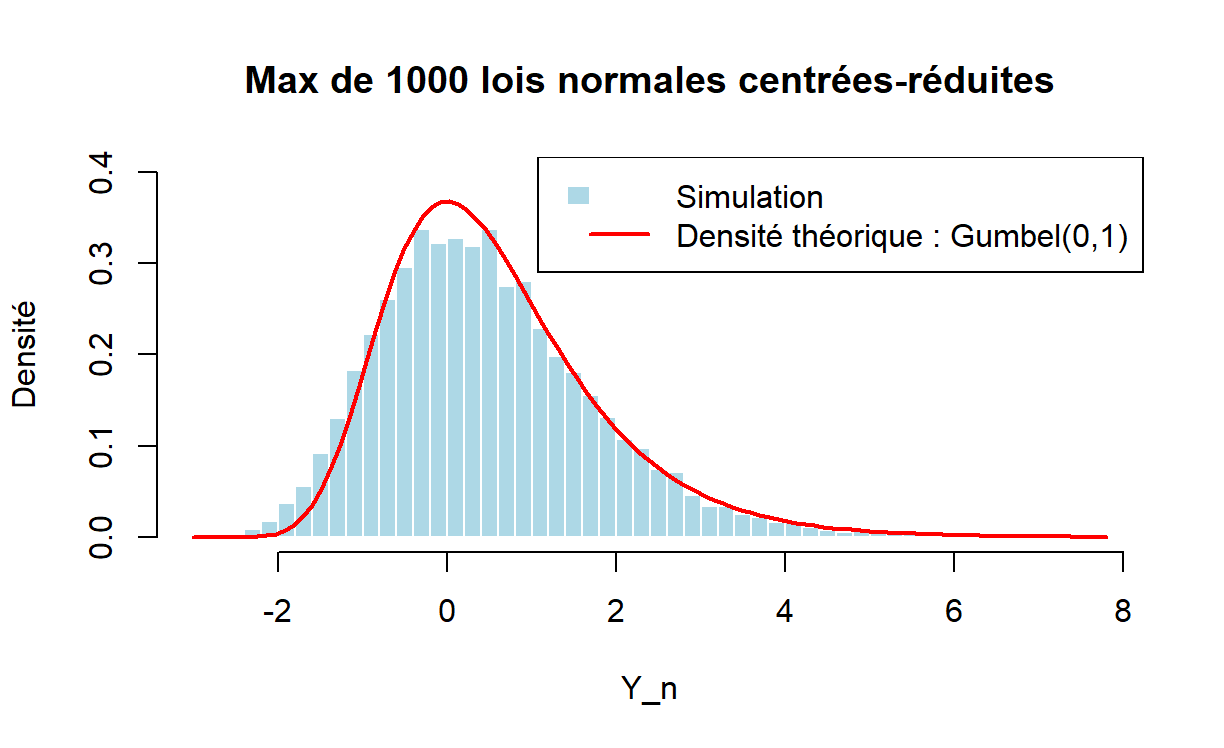
\includegraphics[scale=0.8]{./images/Max_Normale.png} 
\end{center}

\noindent Notons ainsi que l'on a la même loi limite que pour la loi exponentielle de paramètre 1, les graphes sont quasiment identiques.

\subsubsection{Loi de Cauchy}

\noindent Enfin, pour une loi de Cauchy (de paramètres 0 et 1 ici), la loi limite est une loi de Fréchet. On a les coefficients suivants : $a_n = \pi $ et $b_n = n $. \\

\noindent On s'intéresse au comportement asymptotique du maximum $ M_n = \max(X_1, \dots, X_n) $. Pour la loi de Cauchy, on sait que la fonction de répartition est donnée par $ F(x) = \frac{1}{2} + \frac{1}{\pi} \arctan(x) $. Donc, la fonction de survie est $ \bar{F}(x) = 1 - F(x) = \frac{1}{2} - \frac{1}{\pi} \arctan(x) $. \\

\noindent On va utiliser le développement asymptotique suivant, pour \( x \to +\infty \): $\arctan(x) = \frac{\pi}{2} - \frac{1}{x} + o\left(\frac{1}{x}\right) $. \\

\noindent Ainsi, on a $\bar{F}(x) \sim \frac{1}{\pi x} \quad \text{lorsque } x \to +\infty$. \\
\noindent Et donc la loi du maximum \( M_n \) s’écrit alors : $ \mathbb{P}(M_n \leq x) = F(x)^n \xrightarrow[n \to +\infty]{} \left(1 - \frac{1}{\pi x}\right)^n $


\noindent On cherche donc \( a_n > 0 \), \( b_n \) tels que : $ \mathbb{P}\left( \frac{M_n - b_n}{a_n} \leq z \right) \to G(z) = \exp(-1/z) $ où G est la fonction de répartition d'une loi de Fréchet de paramètre 1. \\

\noindent Posons \( b_n = n \), \( a_n = \pi \). Alors :

\[
\mathbb{P}\left( \frac{M_n - n}{\pi} \leq z \right) = \mathbb{P}\left( M_n \leq \pi z + n \right) \xrightarrow[n \to +\infty]{} \left(1 - \frac{1}{\pi(\pi z + n)}\right)^n
\]

\noindent En développant, on obtient : $\left(1 - \frac{1}{\pi(\pi z + n)}\right)^n \xrightarrow[n \to +\infty]{} \exp\left(- \frac{n}{\pi(\pi z + n)} \right)$

\noindent Et lorsque \( n \to \infty \), on a $ \frac{n}{\pi(\pi z + n)} \to \frac{1}{z} $

\noindent Donc : $\mathbb{P}\left( \frac{M_n - n}{\pi} \leq z \right) \to \exp\left(-\frac{1}{z} \right)$ \\

\noindent Ce qui montre que :
\[
\frac{M_n - n}{\pi} \xrightarrow{d} Z \sim \text{Fréchet}(1)
\]


\begin{center}
	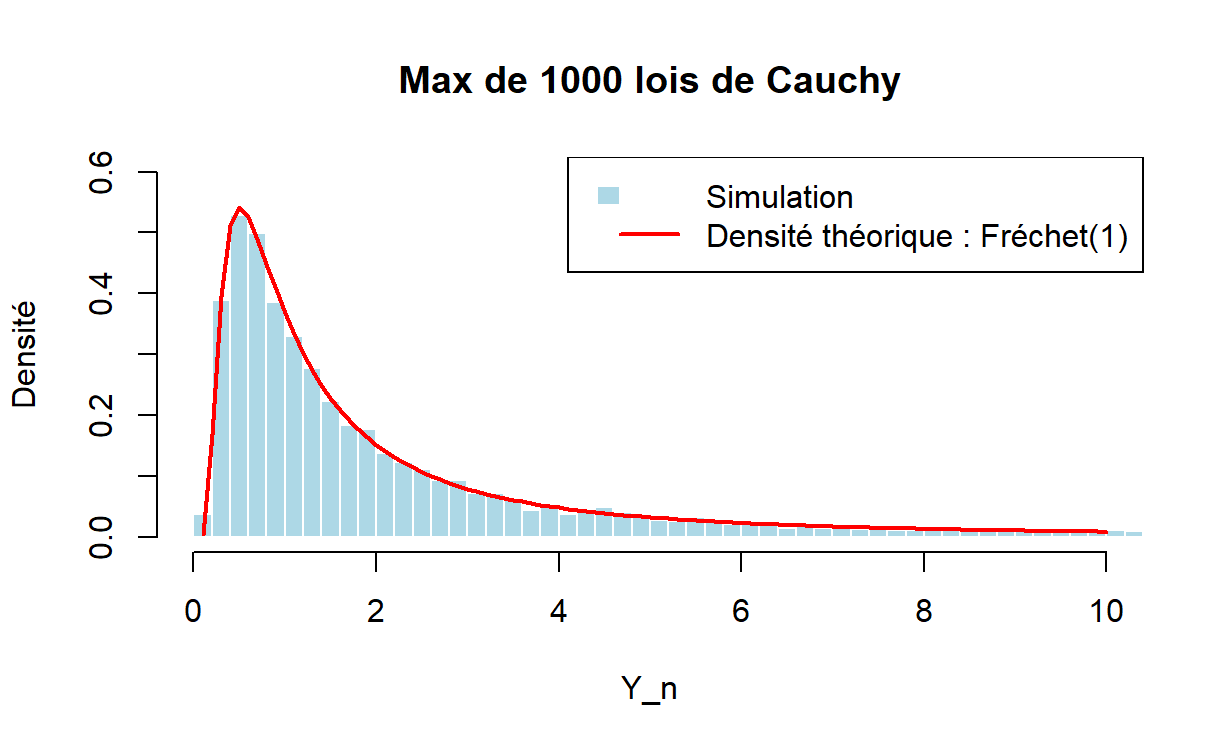
\includegraphics[scale=0.8]{./images/Max_Cauchy.png} 
\end{center}

\noindent Enfin ici, on avait une loi à queue lourde, et on obtient bien la loi de Fréchet attendue.

\newpage

\section{Méthodes d'estimation de l'indice de valeurs extrêmes}
Dans cette section, nous cherchons à estimer le paramètre \(\gamma\) directement à partir des observations \(X_i\), sans nous limiter aux maxima \(M_n\), afin de tirer parti de l’ensemble des données.  
Nous nous concentrons sur deux approches non paramétriques classiques : les estimateurs de Hill et de Pickands. Ces méthodes reposent uniquement sur les statistiques d’ordre et sont particulièrement utilisées en pratique. D'autres estimateurs existent, notamment des versions généralisées ou des approches paramétriques basées sur la vraisemblance ou les moments, mais ils ne seront pas abordés ici. \\

\textbf{Définition :} On appelle \textit{statistique d'ordre} la permutation aléatoire de l'échantillon \(X_1, \dots, X_n\), qui ordonne les valeurs de l’échantillon par ordre croissant :

\[
X_{(1)} \leq X_{(2)} \leq \dots \leq X_{(n)}
\]

\textbf{Définition :} On dit qu'une suite \((k_n)_{n \geq 0}\) d'entiers est intermédiaire si :

\[
\lim_{n \to \infty} k_n = \infty \quad et \lim_{n \to \infty} \frac{k_n}{n} = 0
\]

\textbf{Définition :}
On dit qu'un estimateur \(\hat{\gamma_{n}}\) est convergent s'il converge en probabilité vers \(\gamma\), soit :
\[
\lim_{n \to \infty} P(\lvert \hat{\gamma_{n}} - \gamma \rvert > \epsilon) = 0 \quad \forall \epsilon > 0
\]

\subsection{Estimateur de Pickands}

L’estimateur de Pickands est construit à partir de trois statistiques d’ordre dans un échantillon. Il constitue l’un des premiers estimateurs non paramétriques proposés pour estimer l’indice des valeurs extrêmes \(\gamma\). Son principal avantage réside dans le fait qu’il est valide quel que soit le domaine d’attraction de la loi sous-jacente : Fréchet (\(\xi > 0\)), Gumbel (\(\xi = 0\)) ou Weibull (\(\xi < 0\)). Il n'est donc pas restreint à une famille particulière de distributions et reste applicable dans un cadre très général.

Néanmoins, cet estimateur est connu pour être assez sensible à la taille de l’échantillon, et en particulier au choix du paramètre intermédiaire \(k\), ce qui peut entraîner une certaine instabilité dans les estimations. Cela limite parfois sa robustesse, en particulier pour des tailles d’échantillon modestes.

En 1975, Pickands a démontré la consistance faible de son estimateur, c’est-à-dire la convergence en probabilité vers le vrai paramètre lorsque la taille de l’échantillon tend vers l’infini. Plus tard en 1989, Dekkers et de Haan ont établi la convergence forte ainsi que la normalité asymptotique de cet estimateur sous des conditions plus générales.
\\
\\
\medskip
\textbf{Définition.} Soit \(X_1, \dots, X_n\) une suite de variables aléatoires i.i.d. de loi \(F\), appartenant à l’un des domaines d’attraction des lois de valeurs extrêmes. On note \(X_{1,n} \leq \dots \leq X_{n,n}\) les statistiques d’ordre croissantes. Soit \((k_n)_{n \geq 1}\) une suite intermédiaire telle que \(k_n \to \infty\) et \(k_n / n \to 0\), l’estimateur de Pickands est défini par :

\[
\hat{\gamma}_{k_n,n} = \frac{1}{\ln(2)} \ln\left( \frac{X_{n-k_n +1,n} - X_{n-2k_n +1,n}}{X_{n-2k_n +1,n} - X_{n-4k_n +1,n}} \right)
\]

\medskip
L’estimateur de Pickands repose sur l’idée que, dans les queues d’une distribution extrême, les plus grandes observations suivent un comportement régulier. En considérant des statistiques d’ordre décroissantes, on peut approximer la structure de la queue à l’aide de différences successives entre grandes valeurs. L’utilisation d’une transformation logarithmique permet alors d’isoler l’indice de queue \(\gamma\), sous des conditions d’attraction à une loi limite.

\medskip
\textbf{Propriété de consistance.} Si \((k_n)\) est une suite intermédiaire, alors :
\[
\hat{\gamma}_{k_n,n} \xrightarrow{\mathbb{P}} \gamma
\quad \text{lorsque } n \to \infty.
\]

De plus, sous hypothèses régulières, l’estimateur est asymptotiquement normal :
\[
\sqrt{k_n} \left( \hat{\gamma}_{k_n,n} - \gamma \right) \xrightarrow{\mathcal{L}} \mathcal{N}(0, \sigma^2(\gamma))
\]
où la variance asymptotique est donnée par :
\[
\sigma(\gamma) = \frac{\gamma \sqrt{2^{2\gamma + 1} + 1}}{2(2^{\gamma} - 1)\ln(2)}.
\]

\medskip
Cette formule théorique permet de construire des intervalles de confiance pour l’estimation de \(\gamma\), bien qu’en pratique la variance soit souvent estimée par simulation.

\subsubsection{Construction de l'estimateur de Pickands}

Afin de construire l'estimateur de Pickands, nous allons reprendre la proposition (2.3). Pour \(x,y > 0\) et \(y \neq 1\), la proposition est équivalente à :
\[
\lim_{s \to 0} \frac{U(sx) - U(s)}{U(sy) - U(s)} = 
\begin{cases} 
\frac{x^\gamma - 1}{y^\gamma - 1} & \text{si } \gamma \neq 0, \\
\frac{\log(x)}{\log(y)} & \text{si } \gamma = 0.
\end{cases}
\]
\newline

\begin{lemma}
Soit \(X_1, \dots, X_n\) des variables aléatoires indépendantes et de fonction de répartition \(F\).
Soit \(U_1, \dots, U_n\) des variables aléatoires indépendantes de loi uniforme \(\left[0,1\right]\). Alors \(F^{-1}(U_{1,n}), \dots, F^{-1}(U_{n,n})\) a même loi que \((X_{1,n}, \dots, X_{n,n})\).
\end{lemma}

\begin{proof}
admis
\end{proof}
\noindent On en déduit la construction de l'estimateur de Pickands.
\\
\\
\noindent \textbf{Construction de l'estimateur de Pickands :}

Par la proposition précédente, pour $\gamma \in \mathbb{R}$ et $\alpha$ on a avec le choix $t = 2s$, $x = 2$ et $y = \frac{1}{2}$,
\[
\lim_{t \to \infty} \frac{U(t) - U(t/2)}{U(t/2) - U(t/4)} = 2^{\gamma}.
\]

\noindent En utilisant la croissance de $U$ qui se déduit de la croissance de $F$, on obtient
\[
\lim_{t \to \infty} \frac{U(t) - U(t_{c_1}(t))}{U(t_{c_1}(t)) - U(t_{c_2}(t))} = 2^{\gamma}
\]
dès que $\lim_{t \to \infty} c_1(t) = \frac{1}{2}$ et $\lim_{t \to \infty} c_2(t) = \frac{1}{4}$. Il reste donc à trouver des estimateurs pour $U(t)$.
\\
\\
Soit $k_n,$ pour $ n \geq 1$ une suite d’entiers telle que $1 \leq k_n \leq \frac{n}{4}$ et $\lim_{n \to \infty} \frac{k_n}{n} = 0$ et $\lim_{n \to \infty} k_n = \infty$.
\\
Soit $(V_{1,n},\dots,V_{n,n})$ la statistique d’ordre d’un échantillon de variables aléatoires indépendantes de loi de Pareto. On note $F_V(x) = 1 - x^{-1}, x \geq 1$.
\\
\\
On déduit avec certains résultats de bases liés à $(V_{1,n},\dots,V_{n,n})$ que les suites
\[
\frac{k_n}{n} V_{n-k_n+1,n}, \quad \frac{2k_n}{n} V_{n-2k_n+1,n}, \quad \frac{4k_n}{n} V_{n-4k_n+1,n}
\]
pour \(n \geq 1\) convergent en probabilité vers 1.

On en déduit en particulier, les convergences en probabilité suivantes :
\[
V_{n-k_n+1,n}  \to \infty, \quad \frac{V_{n-2k_n+1,n}}{V_{n-k_n+1,n}} \to \frac{1}{2}, \quad \frac{V_{n-4k_n+1,n}}{V_{n-k_n+1,n}} \to \frac{1}{4}.
\]

Donc la convergence suivante a lieu en probabilité :
\[
\frac{U(V_{n-k_n+1,n}) - U(V_{n-2k_n+1,n})}{U(V_{n-2k_n+1,n}) - U(V_{n-4k_n+1,n})} \to 2^{\gamma}.
\]

Remarquons que si $x \geq 1$, alors $U(x) = F^{-1}(F_V(x))$. On a donc
\[
(U(V_{1,n}), \dots, U(V_{n,n})) = (F^{-1}(F_V(V_{1,n})), \dots, F^{-1}(F_V(V_{n,n}))).
\]

Or \(F_V\) est la fonction de répartition de la loi de Pareto. \newline
On déduit de la croissance de $F_V$ que $(F^{-1}(F_V(V_{1,n})),\dots, F^{-1}(F_V(V_{n,n})))$ a la même loi qu’une suite de $n$ variables aléatoires uniformes sur $[0,1]$ indépendantes. 

On déduit du lemme A que le vecteur aléatoire $(F^{-1}(F_V(V_{1,n})),\dots, F^{-1}(F_V(V_{n,n})))$ a la même loi que $(X_1,\dots,X_n)$. 

Donc la variable aléatoire \(\frac{U(V_{n-k_n+1,n}) - U(V_{n-2k_n+1,n})}{U(V_{n-k_n+1,n}) - U(V_{n-4k_n+1,n})}\) a la même loi que :

\[
\frac{X_{n-k_n+1,n} - X_{n-2k_n+1,n}}{X_{n-k_n+1,n} - X_{n-4k_n+1,n}}
\]

Ainsi cette quantité converge en loi vers $2^{\gamma}$ quand $n$ tend vers l’infini.

\subsubsection{Représentation graphique de l’estimateur de Pickands}

Pour mieux comprendre le comportement de l’estimateur de Pickands dans différents contextes, nous l’appliquons à des données simulées qui sont les mêmes que dans la partie 3, c'est à dire : Pareto, Exponentielle, Uniforme et Cauchy. Ces lois sont choisies pour représenter les trois domaines d’attraction des lois de valeurs extrêmes :

Chaque échantillon comporte $n = 100000$ observations, et l’estimation est faite en fonction de $k$, où \(k\) représente le nombre de plus grandes valeurs utilisées pour estimer l’indice de queue \(\gamma\).

\begin{figure}[H]
    \centering
    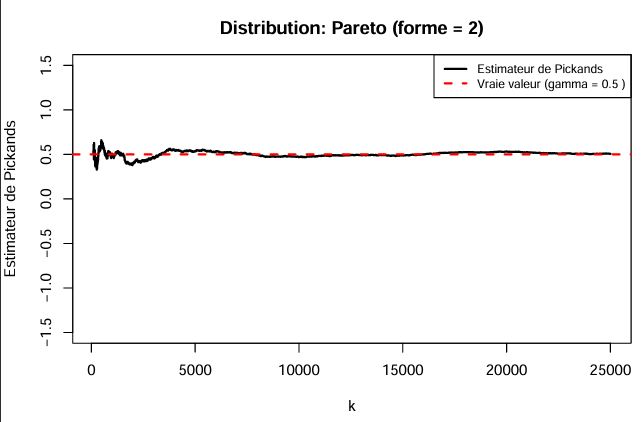
\includegraphics[width=0.6\textwidth]{./image_hill_pickands/pareto_pickands.png}
    \caption{Estimateur de Pickands appliqué à la loi de Pareto ($\gamma = 0.5$)}
\end{figure}
Tout d'abord, pour la loi de Pareto, nous remarquons que l'estimateur de Pickands converge rapidement et de manière stable vers la valeur théorique $\gamma = 0.5$, dès que $k$ devient raisonnablement grand. Cela confirme la bonne performance de l’estimateur pour des lois à queue lourde. On observe cependant une légère variabilité pour les très petites valeurs de $k$, comme attendu.


\begin{figure}[H]
    \centering
    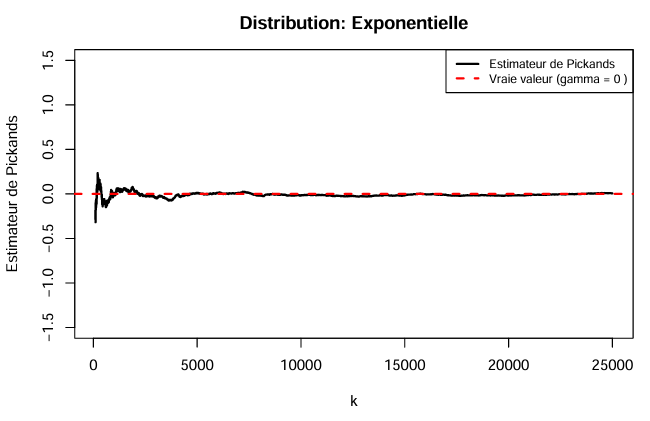
\includegraphics[width=0.6\textwidth]{./image_hill_pickands/exponentielle_pickands.png}
    \caption{Estimateur de Pickands appliqué à la loi Exponentielle ($\gamma = 0$)}
\end{figure}
Dans le cas de la loi exponentielle, qui appartient au domaine de Gumbel, l’estimateur se stabilise très rapidement autour de $\gamma = 0$. Le résultat est ainsi conforme aux attentes.

\begin{figure}[H]
    \centering
    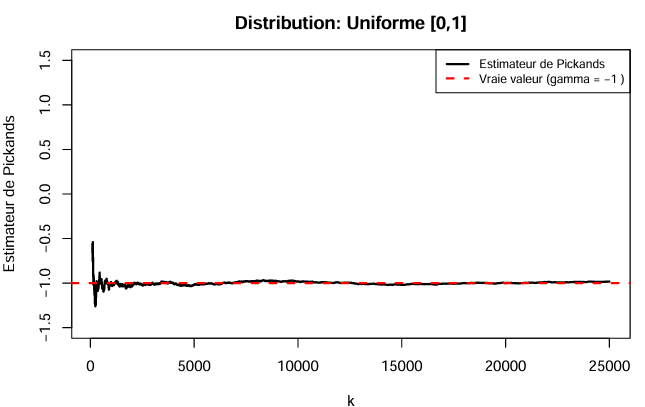
\includegraphics[width=0.6\textwidth]{./image_hill_pickands/uniforme_pickands.png}
    \caption{Estimateur de Pickands appliqué à la loi Uniforme ($\gamma = -1$)}
\end{figure}
Avec la loi uniforme, dont le support est borné, l’estimateur converge vers $\gamma = -1$, ce qui est cohérent avec la théorie. On observe une plus grande variabilité dans les faibles valeurs de $k$, mais une convergence raisonnablement bonne lorsque $k$ augmente.


\begin{figure}[H]
    \centering
    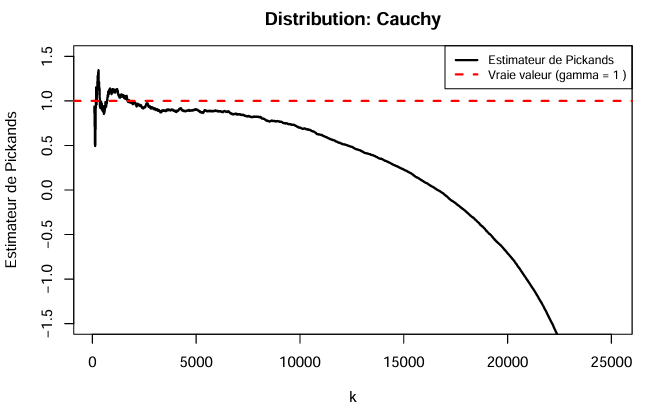
\includegraphics[width=0.6\textwidth]{./image_hill_pickands/cauchy_pickands.png}
    \caption{Estimateur de Pickands appliqué à la loi de Cauchy ($\gamma = 1$)}
\end{figure}
La loi de Cauchy, caractérisée par une queue extrêmement lourde, présente un comportement plus instable. Pour les faibles valeurs de $k$, l’estimateur est instable. Il converge vers $\gamma = 1$ mais, passé un certain seuil (vers $k = 10000$), il commence à décroître, indiquant une dégradation de l’estimation. Cela met en évidence la sensibilité de l’estimateur de Pickands au choix de $k$, en particulier pour des lois aux queues extrêmes. Lorsque trop d'observations non-extrêmes sont incluses, l’estimation devient biaisée.

Ainsi, ces résultats illustrent bien les limites de l’estimateur de Pickands : si \(k\) est trop petit, on observe une forte variance, tandis que si \(k\) est trop grand, l’estimation est biaisée car elle intègre des observations non extrêmes. D’un point de vue théorique, la validité asymptotique de l’estimateur repose sur les conditions suivantes : \(k \to \infty\) et \(k/n \to 0\) lorsque \(n \to \infty\). Cela signifie qu’on doit considérer suffisamment de valeurs extrêmes, tout en veillant à ce que \(k\) reste petit devant \(n\). Dans cette optique, nous limitons volontairement \(k\) à \(n/4\) dans nos simulations, afin de respecter ce cadre théorique et d’éviter que l’estimation ne soit dégradée.


\subsection{Estimateur de Hill}
Cet estimateur a été introduit par Hill en 1975 dans le but d’estimer, de manière non paramétrique, le paramètre de queue des lois appartenant au domaine d’attraction de Fréchet. Il offre une estimation de l’indice de queue généralement plus efficace que celle fournie par l’estimateur de Pickands. La construction de cet estimateur repose sur l’utilisation des $k_n$ plus grandes statistiques d’ordre de l’échantillon.



\subsubsection{La construction de l’estimateur de Hill}
Dans le cadre de l'analyse des valeurs extrêmes, l'estimation de l'indice de queue \(\gamma\) est cruciale pour comprendre le comportement des queues de distribution. L'estimateur de Hill est une méthode largement utilisée pour estimer cet indice de queue.

Soient \(\alpha_n\) et \(\beta_n\) deux suites de nombres positifs. La construction de l'estimateur de Hill repose sur une relation fondamentale entre les quantiles d’une distribution à queue lourde appartenant au domaine d’attraction de Fréchet. Cette relation est donnée par :

\[
    q_{\beta_n} \simeq q_{\alpha_n} \left( \frac{\alpha_n}{\beta_n} \right)^{\gamma}.
\]

Ici, \(q_{\alpha}\) représente le quantile d'ordre \(\alpha\) de la distribution, et \(\gamma\) est l'indice de queue que nous cherchons à estimer. Cette relation exprime que le quantile d'ordre \(\beta_n\) peut être approximé par le quantile d'ordre \(\alpha_n\) multiplié par un facteur dépendant de \(\gamma\).

Pour déterminer l'estimateur de Hill, nous commençons par prendre le logarithme des deux côtés de l'équation du dessus. Nous obtenons :

\[
\log(q_{\beta_n}) - \log(q_{\alpha_n}) \simeq \gamma \log\left( \frac{\alpha_n}{\beta_n} \right).
\]

En posant $\alpha_n = k_n/n$, où \(k_n\) est un nombre d'observations extrêmes que nous considérons, et en prenant plusieurs valeurs pour \(\beta_n\), avec \(\beta_n = i/n\) pour \(i = 1, \ldots, k_n - 1\) et \(\beta_n < \alpha_n\), nous obtenons :

\[
\log(q_{i/n}) - \log(q_{k_n/n}) \simeq \gamma \log(k_n/i).
\]

Ensuite, nous estimons les quantiles par leurs équivalents empiriques, c'est-à-dire les statistiques d'ordre de l'échantillon. Cela conduit à :

\[
\log(X_{n - i + 1, n}) - \log(X_{n - k_n + 1, n}) \simeq \gamma \log(k_n / i).
\]

En sommant sur \(i = 1, \ldots, k_n - 1\), nous obtenons :

\[
\gamma = \frac{\sum_{i=1}^{k_n - 1} \log(X_{n - i + 1, n}) - \log(X_{n - k_n + 1, n})}{\sum_{i=1}^{k_n - 1} \log(k_n / i)}.
\]

Le dénominateur peut être réécrit comme \(\log(k_n^{k_n - 1}/(k_n - 1)!)\). En utilisant la formule de Stirling, nous trouvons que ce dénominateur est équivalent à \(k_n\) au voisinage de l'infini. Cela nous permet d'obtenir l'estimateur de Hill.

Soit $(k_n)_{n \geq 1}$ une suite d'entiers avec $1 \leq k_n \leq n$, l’estimateur de Hill est défini par :

\[
\hat{\gamma}^{H}_{k_n} = \frac{1}{k_n - 1} \sum_{i=1}^{k_n - 1} \log(X_{n - i + 1, n}) - \log(X_{n - k_n + 1, n}).
\]

L’estimateur de Hill satisfait la propriété de consistance faible. Plus précisément, si $(k_n)_{n \geq 1}$ est une suite intermédiaire, alors l’estimateur $\hat{\gamma}^{H}_{k_n}$ converge en probabilité vers le paramètre de queue $\gamma$, c’est-à-dire :
\[
\hat{\gamma}^{H}_{k_n} \xrightarrow{\mathbb{P}} \gamma.
\]

\begin{remark}
	Dans la pratique, déterminer une valeur appropriée pour le paramètre $k_n$, c’est-à-dire le nombre de plus grandes observations à retenir, constitue une étape délicate. Il faut en effet trouver un compromis entre la variance et le biais : utiliser suffisamment de données pour obtenir une estimation fiable, tout en s’assurant que ces données proviennent bien de la queue de la distribution. Diverses approches ont été développées dans la littérature pour guider ce choix.
\end{remark}

\subsubsection{Comportement empirique de l’estimateur de Hill}
Pour analyser le comportement de l’estimateur de Hill, nous l’appliquons à des échantillons simulés de taille $n = 40000$, issus de plusieurs distributions : la loi de Lévy, la loi exponentielle, la loi uniforme sur \([0,1]\), et la loi de Cauchy. Ces distributions couvrent les trois domaines d’attraction des lois de valeurs extrêmes.
Les figures suivantes présentent l’évolution de l’estimateur de Hill en fonction de $k$, le nombre de plus grandes valeurs utilisées. La ligne rouge indique la valeur théorique de $\gamma$, tandis que la courbe noire représente l’estimation, accompagnée d’une bande de confiance à 95\%.
\begin{figure}[H]
    \centering
    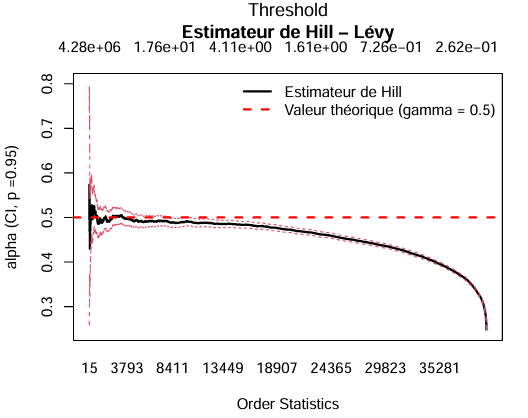
\includegraphics[width=0.55\textwidth]{./image_hill_pickands/levy_hill.png}
    \caption{Estimateur de Hill appliqué à la loi de Lévy ($\gamma = 0.5$)}
\end{figure}
Pour la loi de Lévy, à queue lourde, l’estimateur de Hill converge de manière assez stable vers \(\gamma = 0.5\). Au-delà d’un certain seuil de \(k\), on note cependant une dégradation due à l’inclusion d’observations moins extrêmes.

\begin{figure}[H]
    \centering
    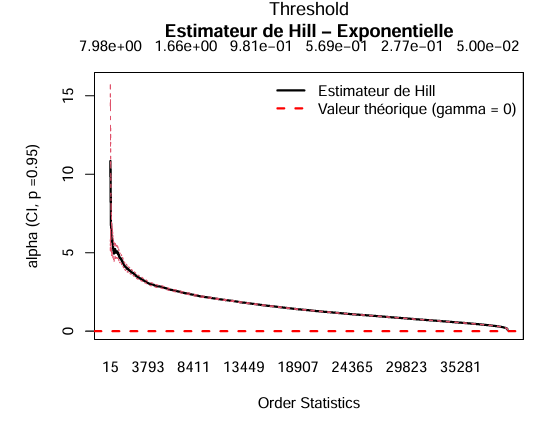
\includegraphics[width=0.55\textwidth]{./image_hill_pickands/exponentielle_hill.png}
    \caption{Estimateur de Hill appliqué à la loi exponentielle ($\gamma = 0$)}
\end{figure}
La loi exponentielle appartient au domaine de Gumbel, avec un indice de queue nul. L’estimateur de Hill n’est pas conçu pour ce cas, ce que montre bien le graphique : les valeurs estimées sont nettement surestimées et décroissent lentement sans atteindre la valeur théorique. Ce comportement traduit l’inadéquation de Hill pour ce type de loi.

\begin{figure}[H]
    \centering
    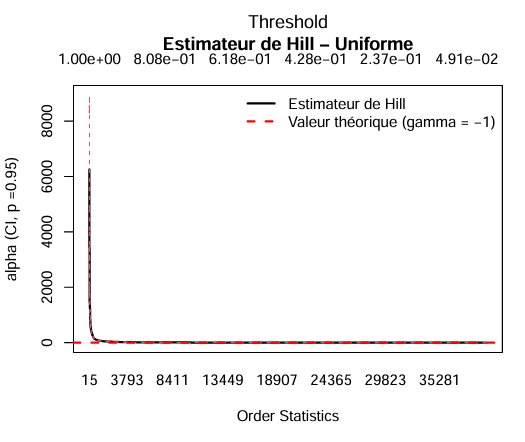
\includegraphics[width=0.55\textwidth]{./image_hill_pickands/uniforme_hill.png}
    \caption{Estimateur de Hill appliqué à la loi uniforme ($\gamma = -1$)}
\end{figure}
La loi uniforme a un support borné et un indice théorique de \(\gamma = -1\), ce qui sort du domaine d’application de Hill, qui suppose \(\gamma > 0\). L’estimateur produit ici des résultats très instables et incohérents, confirmant qu’il ne doit pas être utilisé sur ce type de distribution.

\begin{figure}[H]
    \centering
    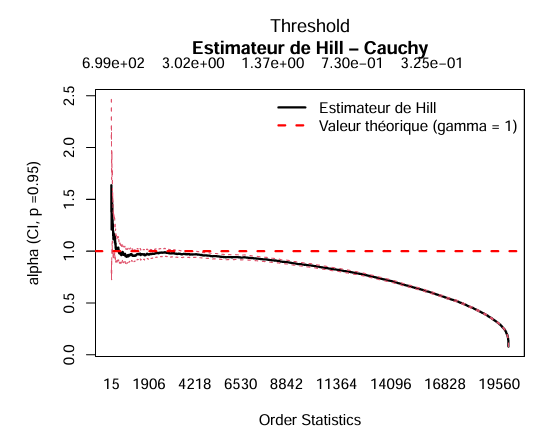
\includegraphics[width=0.55\textwidth]{./image_hill_pickands/cauchy_hill.png}
    \caption{Estimateur de Hill appliqué à la loi de Cauchy ($\gamma = 1$)}
\end{figure}
La loi de Cauchy, avec un indice \(\gamma = 1\), appartient au domaine de Fréchet. L’estimateur fonctionne bien pour de faibles valeurs de \(k\), avec une estimation proche de la valeur théorique. Mais dès que \(k\) devient trop grand, la courbe chute, signe d’un biais induit par les valeurs non extrêmes. Cela illustre la sensibilité de l’estimateur au choix du seuil.

\medskip
\noindent
Ainsi, ces résultats montrent que l’estimateur de Hill est très dépendant du choix du paramètre \(k\), et de la nature de la distribution. Un compromis est nécessaire entre biais (si \(k\) est trop grand) et variance (si \(k\) est trop petit), pour garantir une estimation fiable.


\newpage 
\section{Méthode des maxima par blocs}

\noindent L'approche des maxima par blocs (en anglais Blocks Maxima) consiste à diviser les n observations en N blocs de taille k. Concrètement, la suite $X_1, ..., X_n$ est divisée en N blocs, le premier bloc est $X_1, ..., X_k$, le second $X_{k+1}, ..., X_{2k}$, etc. On obtient ainsi une suite de maxima $M_1, ..., M_n$ définis sur chacun des blocs.\\
\noindent En général, on considère une période temporelle, comme une journée ou bien une année pour refléter le sens des observations.  \\
\noindent On peut alors déterminer la loi limite des maxima, en vertu du théorème de Fisher-Tippett-Gnedenko c'est une distribution GEV classique de la forme :
\[
G_{\mu,\sigma,\gamma}(x)
\;=\;
\exp\!\Bigl\{-\bigl[1 + \gamma\,u\bigr]^{-1/\gamma}\Bigr\}.
\]

\noindent De la même manière que ce que l'on avait sans les blocs, il faut alors déterminer les valeurs des paramètres en les approximant par des méthodes comme le maximum de vraisemblance. Des auteurs comme Ferreira et de Haan (2006 et 2015) ont alors démontré l'existence d'estimateurs pertinents pour cette méthode, nommés PWM (pour "probability weighted moment"). Pour les définir, on part de la statistique suivante, soient $X_{1,k}, ..., X_{k,k}$ les observations ordonnées du bloc $X_1, ..., X_k$, on définit :
\[
\beta_r = \frac{1}{k} \sum_{i=1}^{k} \frac{(i-1)...(i-r)}{(k-1)...(k-r)} X_{i,k} ~ \text{ pour $r = 1,2,3,...,k>r $}
\] \\
\noindent A partir de $\beta_r$, on peut ensuite définir les trois estimateurs PVM suivants pour $\gamma, a_n$ et $b_n$ qui possèdent de bonnes propriétés asymptotiques sous certaines conditions ($\Gamma$ est la fonction gamma d'Euler). \\

\noindent Pour $\gamma$ : $\hat{\gamma}_{k,m}$ est solution de $\frac{3\hat{\gamma}_{k,m} - 1}{2\hat{\gamma}_{k,m} - 1} = \frac{3\beta_2 - \beta_0}{2\beta_1 - \beta_0} $ \\
\noindent Pour $a_n$ : $\hat{a}_{k,m} = \frac{\hat{\gamma}_{k,m}}{2\hat{\gamma}_{k,m} - 1} \cdot \frac{2\beta_1 - \beta_0}{\Gamma(1 - \hat{\gamma}_{k,m})}$ \\
\noindent Pour $b_n$ : $\hat{b}_{k,m} = \beta_0 + \hat{a}_{k,m} \cdot \frac{1 - \Gamma(1 - \hat{\gamma}_{k,m})}{\hat{\gamma}_{k,m}}$ \\

\noindent Sous certaines conditions, on peut enfin démontrer que les quantiles élevés sont estimables par cette méthode. On a ainsi :
\[
\frac{\sqrt{k} \left( \hat{X}_{k,m} - X_n \right)}{a_n \, q_{\gamma}(c_n)}
\xrightarrow{d}
\Delta + (\gamma^-)^2 B - \gamma^- \Lambda - \lambda \frac{\gamma^-}{\gamma^- + \rho}
\]
où : \begin{itemize}
	\item $\hat{X}_{k,m}$ est l’estimateur du quantile extrême
	\item $X_n$ est le vrai quantile à estimer
	\item $a_n$ est le paramètre d'échelle
	\item $\Delta, \Lambda, \lambda$ sont des paramètres issus de la théorie asymptotique de Ferreira et de Haan (2015)
	\item $B$ est un pont brownien
	\item $q_{\gamma}(c_n)$ est une fonction définie par $q_{\gamma}(t) = \int_1^t s^{\gamma - 1} \log s \, ds$
	\item $\gamma^- = \min(0, \gamma)$
\end{itemize}
\vspace{0.5cm}
\noindent Cette approche possède tout de même un défaut car lorsque l'on prend le maximum sur un bloc, on fait potentiellement disparaître des valeurs élevées, on perd des données intéressantes.

\subsection{quantile de retour}

En pratique, on cherche une valeur qui donnerait une certaine confiance quand à l'apparition
de données la depassant. Dans le cas d'une distribution à queue bornée il suffit de prendre la bornes supérieure de la distribution.
\\
Or, dans le cas d'une distribution à queue lourde et exponentiel ce n'est pas possible. On introduit alors la notion de \textbf{quantile de retour} qui est une valeur que l'on dépasse en moyenne une fois tous les T ans.
\\
On pose $z_T$ cette quantité, et elle est solution de l'équation suivante :
\[
P\bigl(M \le z_T\bigr)
\;=\;
G_{\mu,\sigma,\gamma}(z_T)
\;=\;
1 - \frac{1}{T},
\]
où \(G_{\mu,\sigma,\gamma}\) est la fonction de répartition de la GEV. En résolvant cette équation que l'on admet, on obtient
\[
z_T =
\begin{cases}
\displaystyle
\mu \;+\;\frac{\sigma}{\gamma}\Bigl[(-\ln(1 - 1/T))^{-\gamma} - 1\Bigr],
&\gamma \neq 0,\\[1em]
\displaystyle
\mu \;-\;\sigma\,\ln\bigl(-\ln(1 - 1/T)\bigr),
&\gamma = 0.
\end{cases}
\]
\\
\\
\section{Méthode des excès}

La méthode des excès, également appelée approche par dépassement de seuil (en anglais \textit{Peaks Over Threshold}, ou POT), a été introduite par Pickands en 1975. Elle constitue une alternative à l’approche classique par blocs pour modéliser les phénomènes extrêmes.

Le principe est de ne conserver que les observations excédant un seuil élevé \( u \). Si ce seuil est bien choisi la distribution des excès définis par :
\[
Y_i = X_i - u \quad \text{pour} \quad X_i > u
\]
peut être approximée par une distribution de Pareto généralisée (GPD).

\medskip
Cette approche repose sur un résultat fondamental de Balkema et de Haan (1974), et de Pickands (1975), selon lequel, pour une grande classe de lois de probabilité \(F\), la loi des excès conditionnels au-delà d’un seuil élevé converge vers une loi de Pareto généralisée lorsque le seuil \(u\) tend vers la borne supérieure de \(F\).

\medskip
Formellement, on considère une suite de variables aléatoires i.i.d. \(X_1, \dots, X_n\) de fonction de répartition \(F\), et \(x_F\) le point terminal de \(F\). Pour tout seuil \(u < x_F\), on définit la fonction de répartition des excès par :

\[
F_u(x) := \mathbb{P}(X - u \leq x \mid X > u) = \frac{F(x + u) - F(u)}{1 - F(u)},
\quad \text{pour } 0 \leq x \leq x_F - u.
\]

Et sa version en fonction de survie :
\[
\overline{F}_u(x) := \mathbb{P}(X - u > x \mid X > u) = \frac{\overline{F}(x + u)}{\overline{F}(u)}.
\]

Lorsque le seuil \(u\) est suffisamment élevé, \(F_u\) peut être bien approchée par une distribution de Pareto généralisée \(G_{\gamma, \beta(u)}\), définie comme suit :

\subsection{Loi de Pareto généralisée (GPD)}

La fonction de répartition de la GPD est donnée par :

\[
G_{\gamma, \beta}(y) =
\begin{cases}
1 - \left(1 + \dfrac{\gamma y}{\beta}\right)^{-1/\gamma}, & \text{si } \gamma \neq 0, \\
1 - \exp\left(-\dfrac{y}{\beta}\right), & \text{si } \gamma = 0,
\end{cases}
\]
avec \( y \geq 0 \), sous la condition \(1 + \gamma y/\beta > 0\). Le paramètre \(\beta > 0\) représente l’échelle et \(\gamma\) le paramètre de forme (indice de queue).

\medskip
\textbf{Exemple (cas exponentiel)}.\\
Soit \(F(x) = 1 - e^{-x}\) la loi exponentielle standard. On a pour tout \(y > 0\) :

\[
\mathbb{P}(X - u > y \mid X > u) = \frac{e^{-(u + y)}}{e^{-u}} = e^{-y}.
\]

On retrouve donc une loi exponentielle, qui correspond à une GPD avec \(\gamma = 0\) et \(\beta = 1\). Cela montre que l’exponentielle est un cas particulier de GPD.

\subsection{Théorème de Balkema–de Haan–Pickands}

Le résultat central qui justifie l’utilisation de la GPD pour modéliser les excès est le suivant :

\begin{quote}
Soit \(F\) une fonction de répartition appartenant au domaine d’attraction d’une loi de valeur extrême \(\mathcal{H}_\gamma\). Alors, lorsque \(u \to x_F\), il existe une fonction \(\beta(u)\) telle que :
\[
\sup_{0 \leq x \leq x_F - u} \left| F_u(x) - G_{\gamma, \beta(u)}(x) \right| \to 0.
\]
\end{quote}

Autrement dit, plus le seuil \(u\) est élevé, plus la loi des excès au-dessus de ce seuil est bien approchée par une GPD.

\medskip
Cette propriété est essentielle en statistique des valeurs extrêmes, car elle permet d’exploiter pleinement les données situées dans les queues de distribution, sans se limiter au maximum d’un bloc.
\newpage
\section{Application sur des données réelles}
\subsection{Description des données}

Afin d'illustrer les méthodes d'estimation de l'indice de valeurs extrêmes, nous allons appliquer ces techniques sur des données réelles.
Nous allons utiliser les données du package $ismev$ de R. Plus précisément celui de rain et de danish. Ils contienent respectivement les données de pluie journalière en Angleterre de 1914 à 1962 et 
les grands sinistres incendie survenus au Danemark entre 1980 et 1990.
\\
\\
L'objectif sur ces données est de savoir s'il existe (et le cas échéant de le calculer) un seuil tel que à l'avenir on dépasse cette valeur rarement tout en restant raisonable.

\begin{center}
	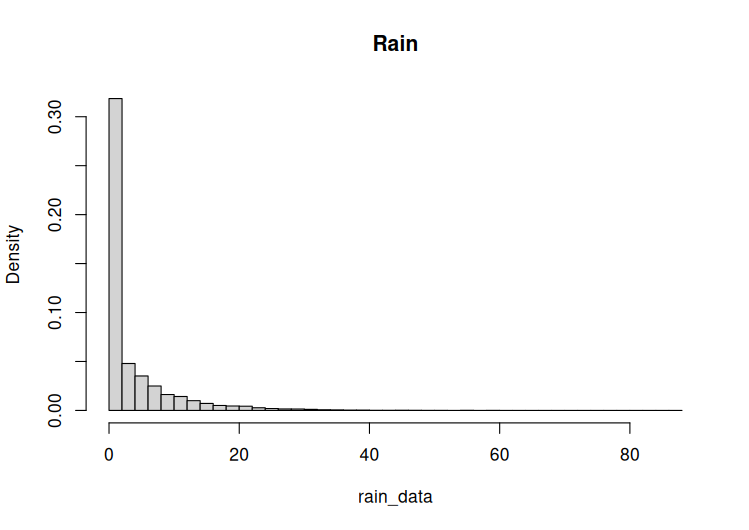
\includegraphics[scale=0.70]{./images/rainhisto.png} 
\end{center}

Dans le cas de rain, on remarque que les données sont concentrées autour de 0 mais qu'elles sont capables de prendre des valeurs très élevées jusqu'à 90.
Il est alors raisonnable de penser qu'après estimation, on va obtenir une valeur de gamma positive ou nulle. En effet, il n'apparait pas de cassure dans la distribution des données.
De plus, les données prennent des valeurs grandes mais perdent rapidement en densité pour celle-ci. Ce qui suggèrerait une valeur de gamma proche de $0$ et positive.

\begin{center}
	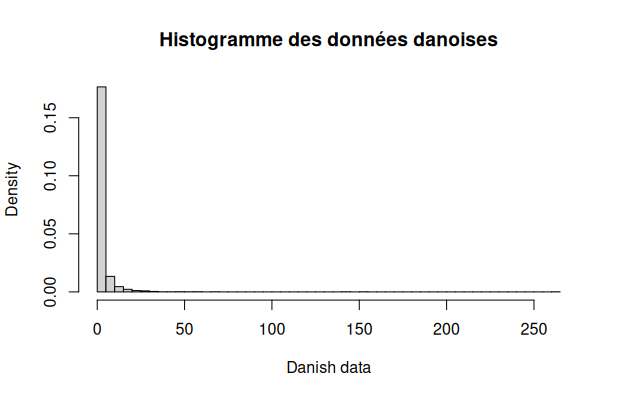
\includegraphics[scale=0.70]{./images/sinistres.png} 
\end{center}

De même, pour les sinistres, on remarque que la majorité des sinistres sont de faible intensité mais qu'il existe des sinistres de grande intensité. On peut donc s'attendre à une valeur de gamma positive ou nulle.

\subsection{Méthode des maxima par bloc}

\subsubsection{Application sur les données de Rain}

Les données étant journalières, on va choisir des blocs de taille 365, comme les données vont de 1914 à 1962, on se retrouve avec 48 blocs de 365 jours.
\\
\\
Via le package \textbf{evd}, on obtient via une estimations par maximum de vraisemblance les paramètres suivants :
\\
$\mu = 40,8$, $\sigma = 9,73$ et $\gamma = 0,107$.
\\
L'estimation des paramètres sont calculées par l'algorithme de Nelder-Mead (voir annexe).
\\
\\
On suppose alors que $\gamma \geq 0$, donc il n’existe pas de valeur maximale finie : la probabilité de très gros maxima décroît mais n'est pas finie, selon un comportement polynomial ou exponentiel ce qui est embettant dans le cas pratique surtout quand on cherche des seuils rarement atteints.
\subsubsection{Application sur les données danish}
On applique la même méthode sur les données de sinistres mais avec une approche légèrement différente puisque les données ne sont pas dans le même format. En effet, on ne dispose pas de données journalières mais l'ensemble des sinistres sur une période de 10 ans. C'est à dire qu'il existe des jours sans sinistres qui ne sont pas comptabilisés.
On regroupe alors les sinistres par mois et on prend le montant de sinistre le plus élevé. On se retrouve alors avec des blocs de taille irrégulière.
\\
\\
Après analyse numérique par maximum de vraisemblance, on obtient les paramètres suivants : $\mu = 8,376$, $\sigma = 5,971$ et $\gamma = 0,623$.
\\
\\
On possède une valeur de gamma positive ce qui renforce l'hypothèse d'une queue lourde pour la distribution du max.

\subsubsection{Synthèse sur la méthode des maxima en bloc}

Quand on dispose des données sur une longue période, la méthode des maxima en bloc est efficace. D'autant plus quand on a des données temporelles (journalières, mensuelles, annuelles).
En revanche, elle utilise moins de données ce qui la rend plus difficile à utiliser en pratique. En effet, on ne garde que les maximums et on perd donc une partie des données qui peuvent etre consequents en fonction du choix de $k$.
Par ailleurs, le choix de $k$ est important car il faut choisir un nombre de blocs suffisant pour avoir une estimation fiable mais pas trop grand pour ne pas perdre trop d'informations.

\subsection{Méthode de dépassement de seuil}


\subsubsection{Application sur les données de Rain}

On a calculé la valeur de $\gamma$ par la méthode des maxima en bloc et obtenu une valeur de $\gamma > 0 $ mais proche de 0. On souhaite s'assurer du signe de $\gamma$
en procédant par la méthode de dépassement de seuil.
\\
On decide de prendre un seuil correspondant au quantile d’ordre 0,95.
\\
\\
On obtient numériquement : 
$\gamma  = -0.027$
\\
\\
On a obtenu dans la méthode des maxima en bloc une valeur de $\gamma$ postive mais proche de 0,
tandis qu'avec la méthode de dépassement de seuil, on obtient une valeur négative mais tout aussi proche de 0.
\\
Ce qui nous amène à conclure que la valeur de $\gamma$ est de 0.
\\
Autrement dit, la distribution du maximum de pluie suit une loi de Gumbel.
\\
\\
On peut néamoins donner une valeur "seuil" qui nous assurerait que la probabilité de dépasser cette valeur est très faible. 
On calcule alors le quantile de retour pour $T=100$ afin d'avoir une valeur de pluie qui ne devrait pas être dépassée plus d'une fois tous les 100 ans.
\\
\\
Dans notre cas, on obtient alors : $z_t = 98,636$. Autrement dit, une fois tous les 100 ans, on peut s'attendre à avoir une pluie de plus de 98.636 mm.

\subsubsection{Application sur les données danish}

On prend un seuil correspondant au quantile d’ordre 0,95. Apres calcul numérique, on obtient $\sigma = 7.038$ et $\gamma = 0.492$.
\\
On a obtenue une valeur de $\gamma$ positive ce qui renforce l'hypothèse d'une queue lourde pour la distribution du max, ce qui est cohérent avec la méthode des maxima en bloc. On peut pousser l'analyse de $\gamma$ en calculant son estimation via l'estimateur de Hill afin d'avoir une valeur plus précise.
\\
\\
On trace alors la courbe de l'estimateur de Hill en fonction de $k$.

\begin{center}
	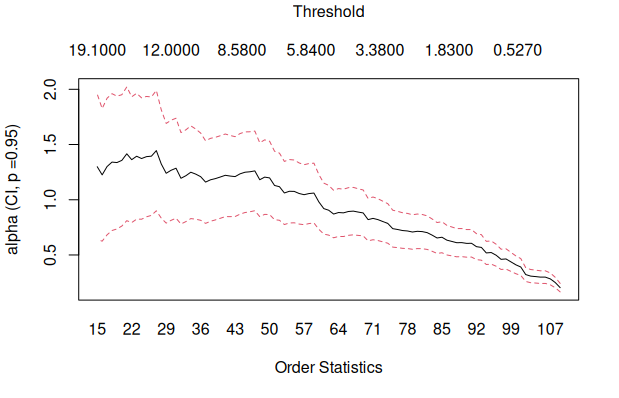
\includegraphics[scale=0.70]{./images/danishsad.png} 
\end{center}

On observe alors un plateau pour k entre 30 et 45. On obtient alors apres estimation numérique une valeur de $\gamma = 0,66$.
\\
On peut alors calculer le quantile de retour pour $T=50$ afin d'avoir une valeur de sinistre qui ne devrait pas être dépassée plus d'une fois tous les 50 ans.
\\
On obtient alors : $z_t = 515,22$. Autrement dit, une fois tous les 50 ans, on peut s'attendre à avoir un sinistre depassant plus de $515,22$.

\subsubsection{Synthèse sur la méthode de dépassement de seuil}
Cette méthode à le bont goût d'exploiter toutes les valeurs supérieures à un seuil, pas seulement un maximum par bloc. Elle utilise donc plus de données.
\\
En revanche le choix du seuil est important car il faut choisir un seuil suffisamment élevé pour ne pas avoir trop peu de données mais pas trop élevé pour ne pas perdre d'informations sur les max. Il faut donc faire le compromis entre le biais et la variance.

\newpage
\section{Annexe}
\subsection{Quelques simulations pour les méthodes de maxima par blocs et dépassement de seuil}

\noindent Quelques illustrations simulées des méthodes vues dans le texte pour les lois uniforme, normale et de Cauchy. \\

\subsubsection{Maxima par blocs}

\begin{center}
	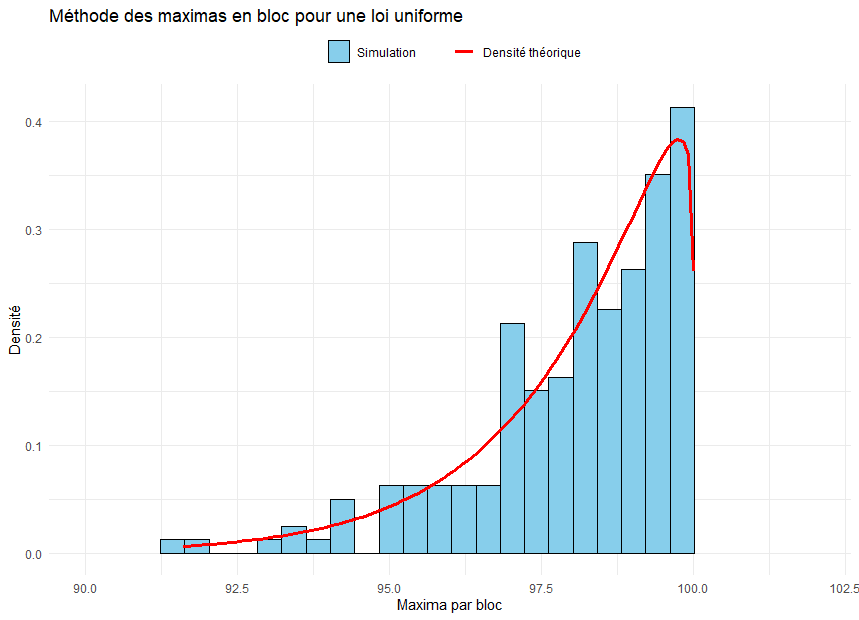
\includegraphics[scale=0.60]{./images/MB_Uniforme} 
\end{center}

\begin{center}
	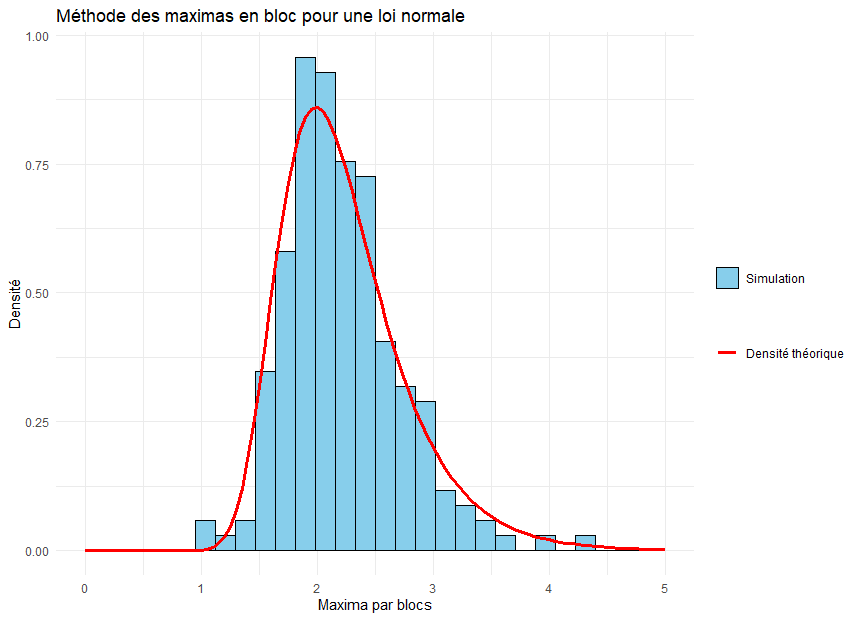
\includegraphics[scale=0.70]{./images/MB_Normale} 
\end{center}

\begin{center}
	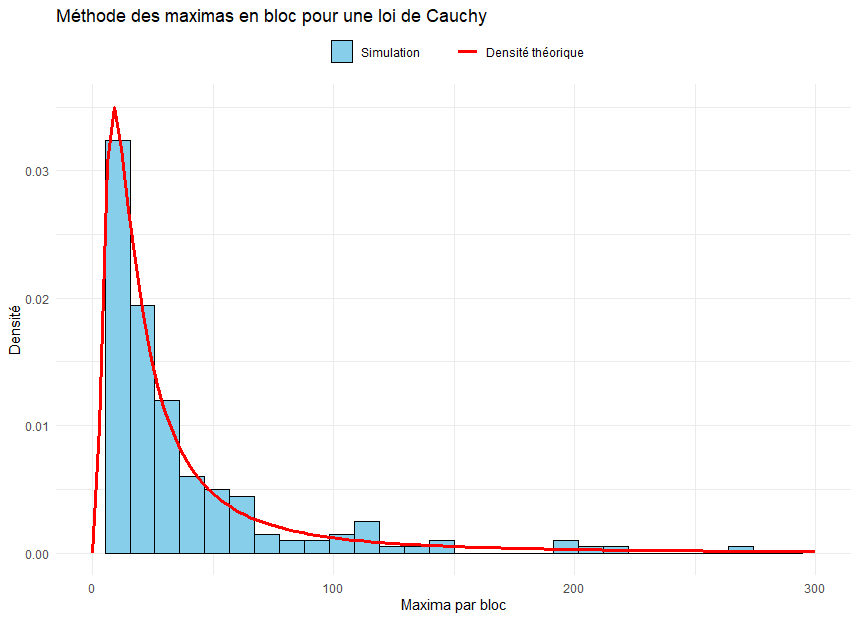
\includegraphics[scale=0.70]{./images/MB_Cauchy} 
\end{center}

\subsubsection{Dépassements de seuil}

\begin{center}
	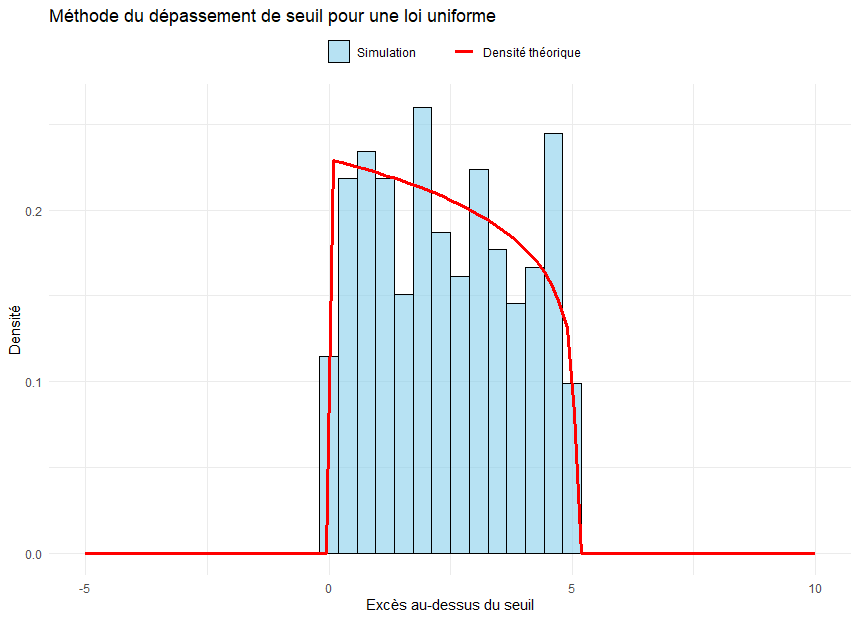
\includegraphics[scale=0.70]{./images/DS_Uniforme} 
\end{center}

\begin{center}
	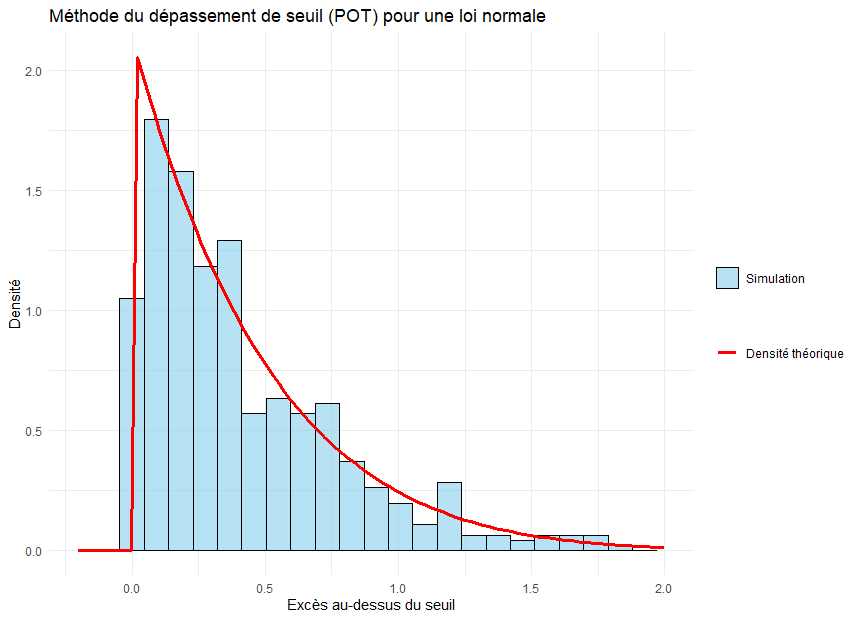
\includegraphics[scale=0.70]{./images/DS_Normale} 
\end{center}

\begin{center}
	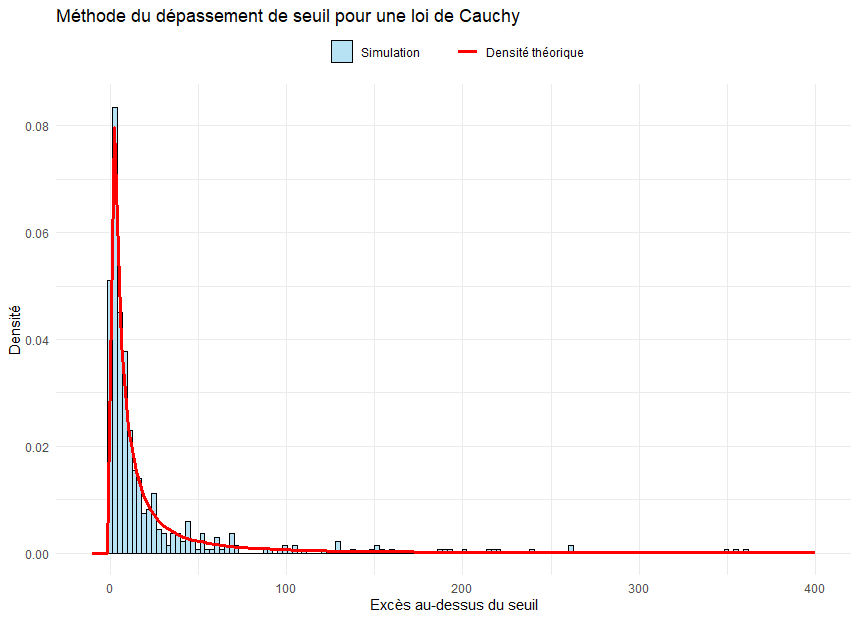
\includegraphics[scale=0.70]{./images/DS_Cauchy} 
\end{center}

\subsection{Codes R}

\noindent Le code pour pour les sorties graphiques et les calculs des estimateurs sont disponible sur le github du projet : https://github.com/DamienMariac/HAX817X-Projet.

\newpage
\section{Bibliographie}

\begin{itemize}
	\item An Introduction to Statistical Modeling of Extreme Values, Stuart Coles 2001
	\item Modelling Extremal Events  Paul Embrechts , Claudia Klüppelberg , Thomas Mikosch
	\item Statistics of Extremes Theory and Applications, Jan Beirlant, Yuri Goegebeur, Johan Segers, Jozef Teugels
	\item Bibm@th.net
\end{itemize}

\end{document}